\documentclass[../rapport.tex]{subfiles}
\graphicspath{{\subfix{ressources/photos_diagrammes/extensionThomas/}}}

\begin{document}
		\subsubsection{Vue d'ensemble}
		Le but de cette extension est de rajouter la gestion de contrats d'assurances divers
		à la fois pour les client smais égalemet pour les insitutions. L'extension se base tout
		de même sur la structure de l'application 1 car c'est dans celle-ci qu'elle la plus 
		utilisée. En effet, dans l'appliction 2 elle est gére comme les autres produits 
		financiers. Il n'y a réellement que la réponse à une demande de devis qui diffère.
		Afin de rendre les diagrammes plus visibles j'ai changé les couleurs des éléments rajoutés. 
		Rose pour le diagramme d'entité relation et jaune pour les autres diagrammes.

		\subsubsection{Application 1}

		\subsubsection{Diagramme des cas d'utilisation}
				\begin{figure}[h]
						\centering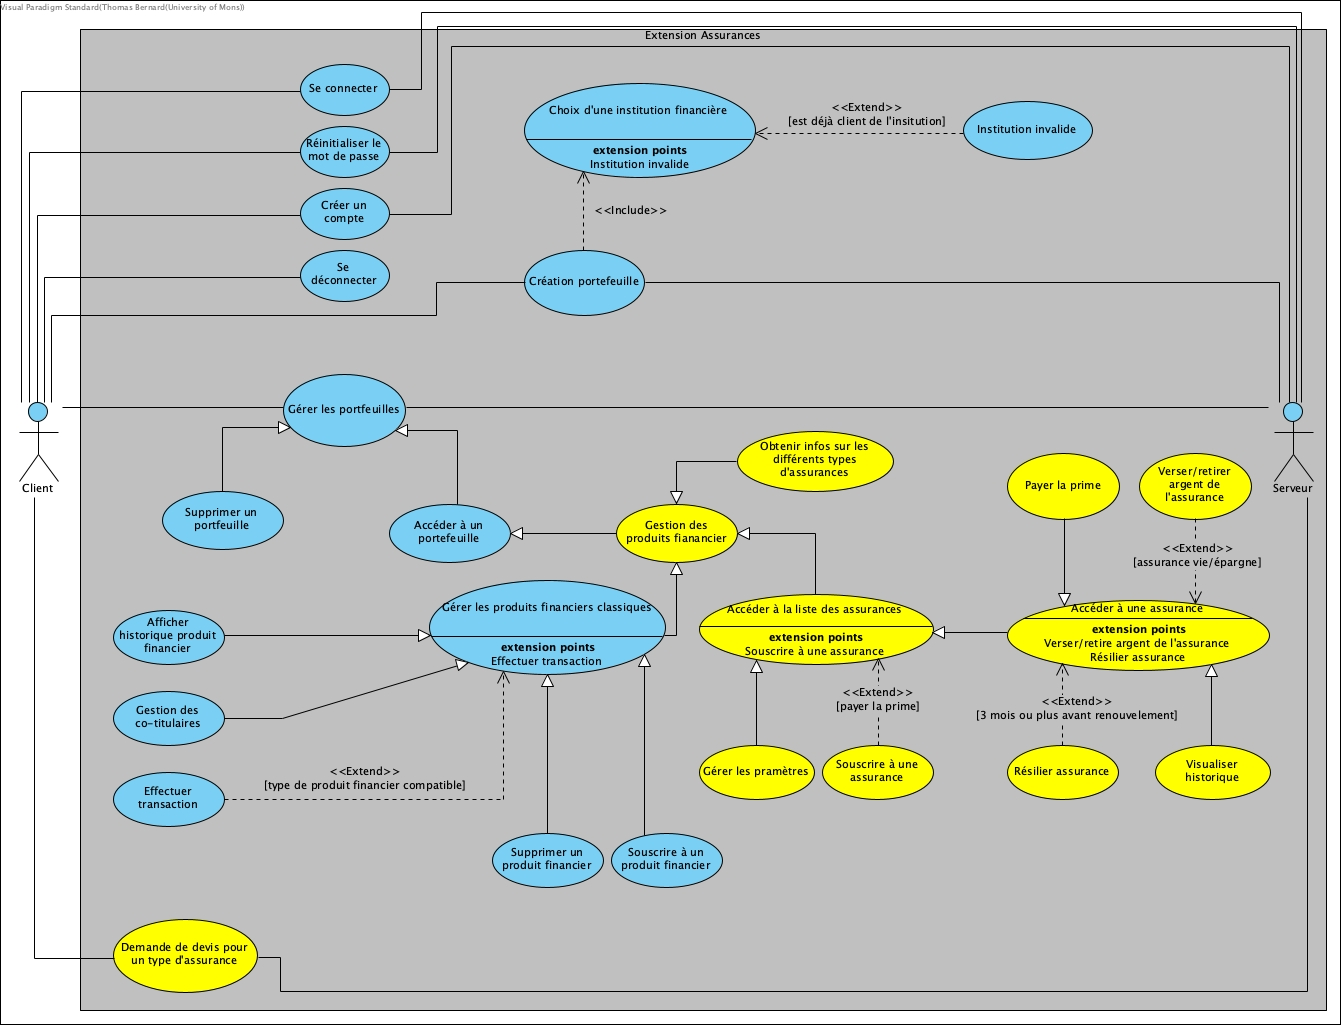
\includegraphics[scale=0.27]{ressources/photos_diagrammes/extensionThomas/useCase1Thomas.jpg}
						\caption{Diagramme des cas d'utilisation de l'app 1 avec extension}
				\end{figure}
		J'ai rajouté un ensemble de divers cas d'utilisations qui sont propres aux assurances
		mais toutefois semblables aux cas d'utilisation relatifs aux produits financiers
		classiques. Il n'y a aucune remarque particulière à faire concernant les cas
		d'utilisation car le modèle est calqué sur le diagramme de base.
\newpage
		\subsubsection{Interaction Overview Diagram}
				\begin{figure}[h]
						\centering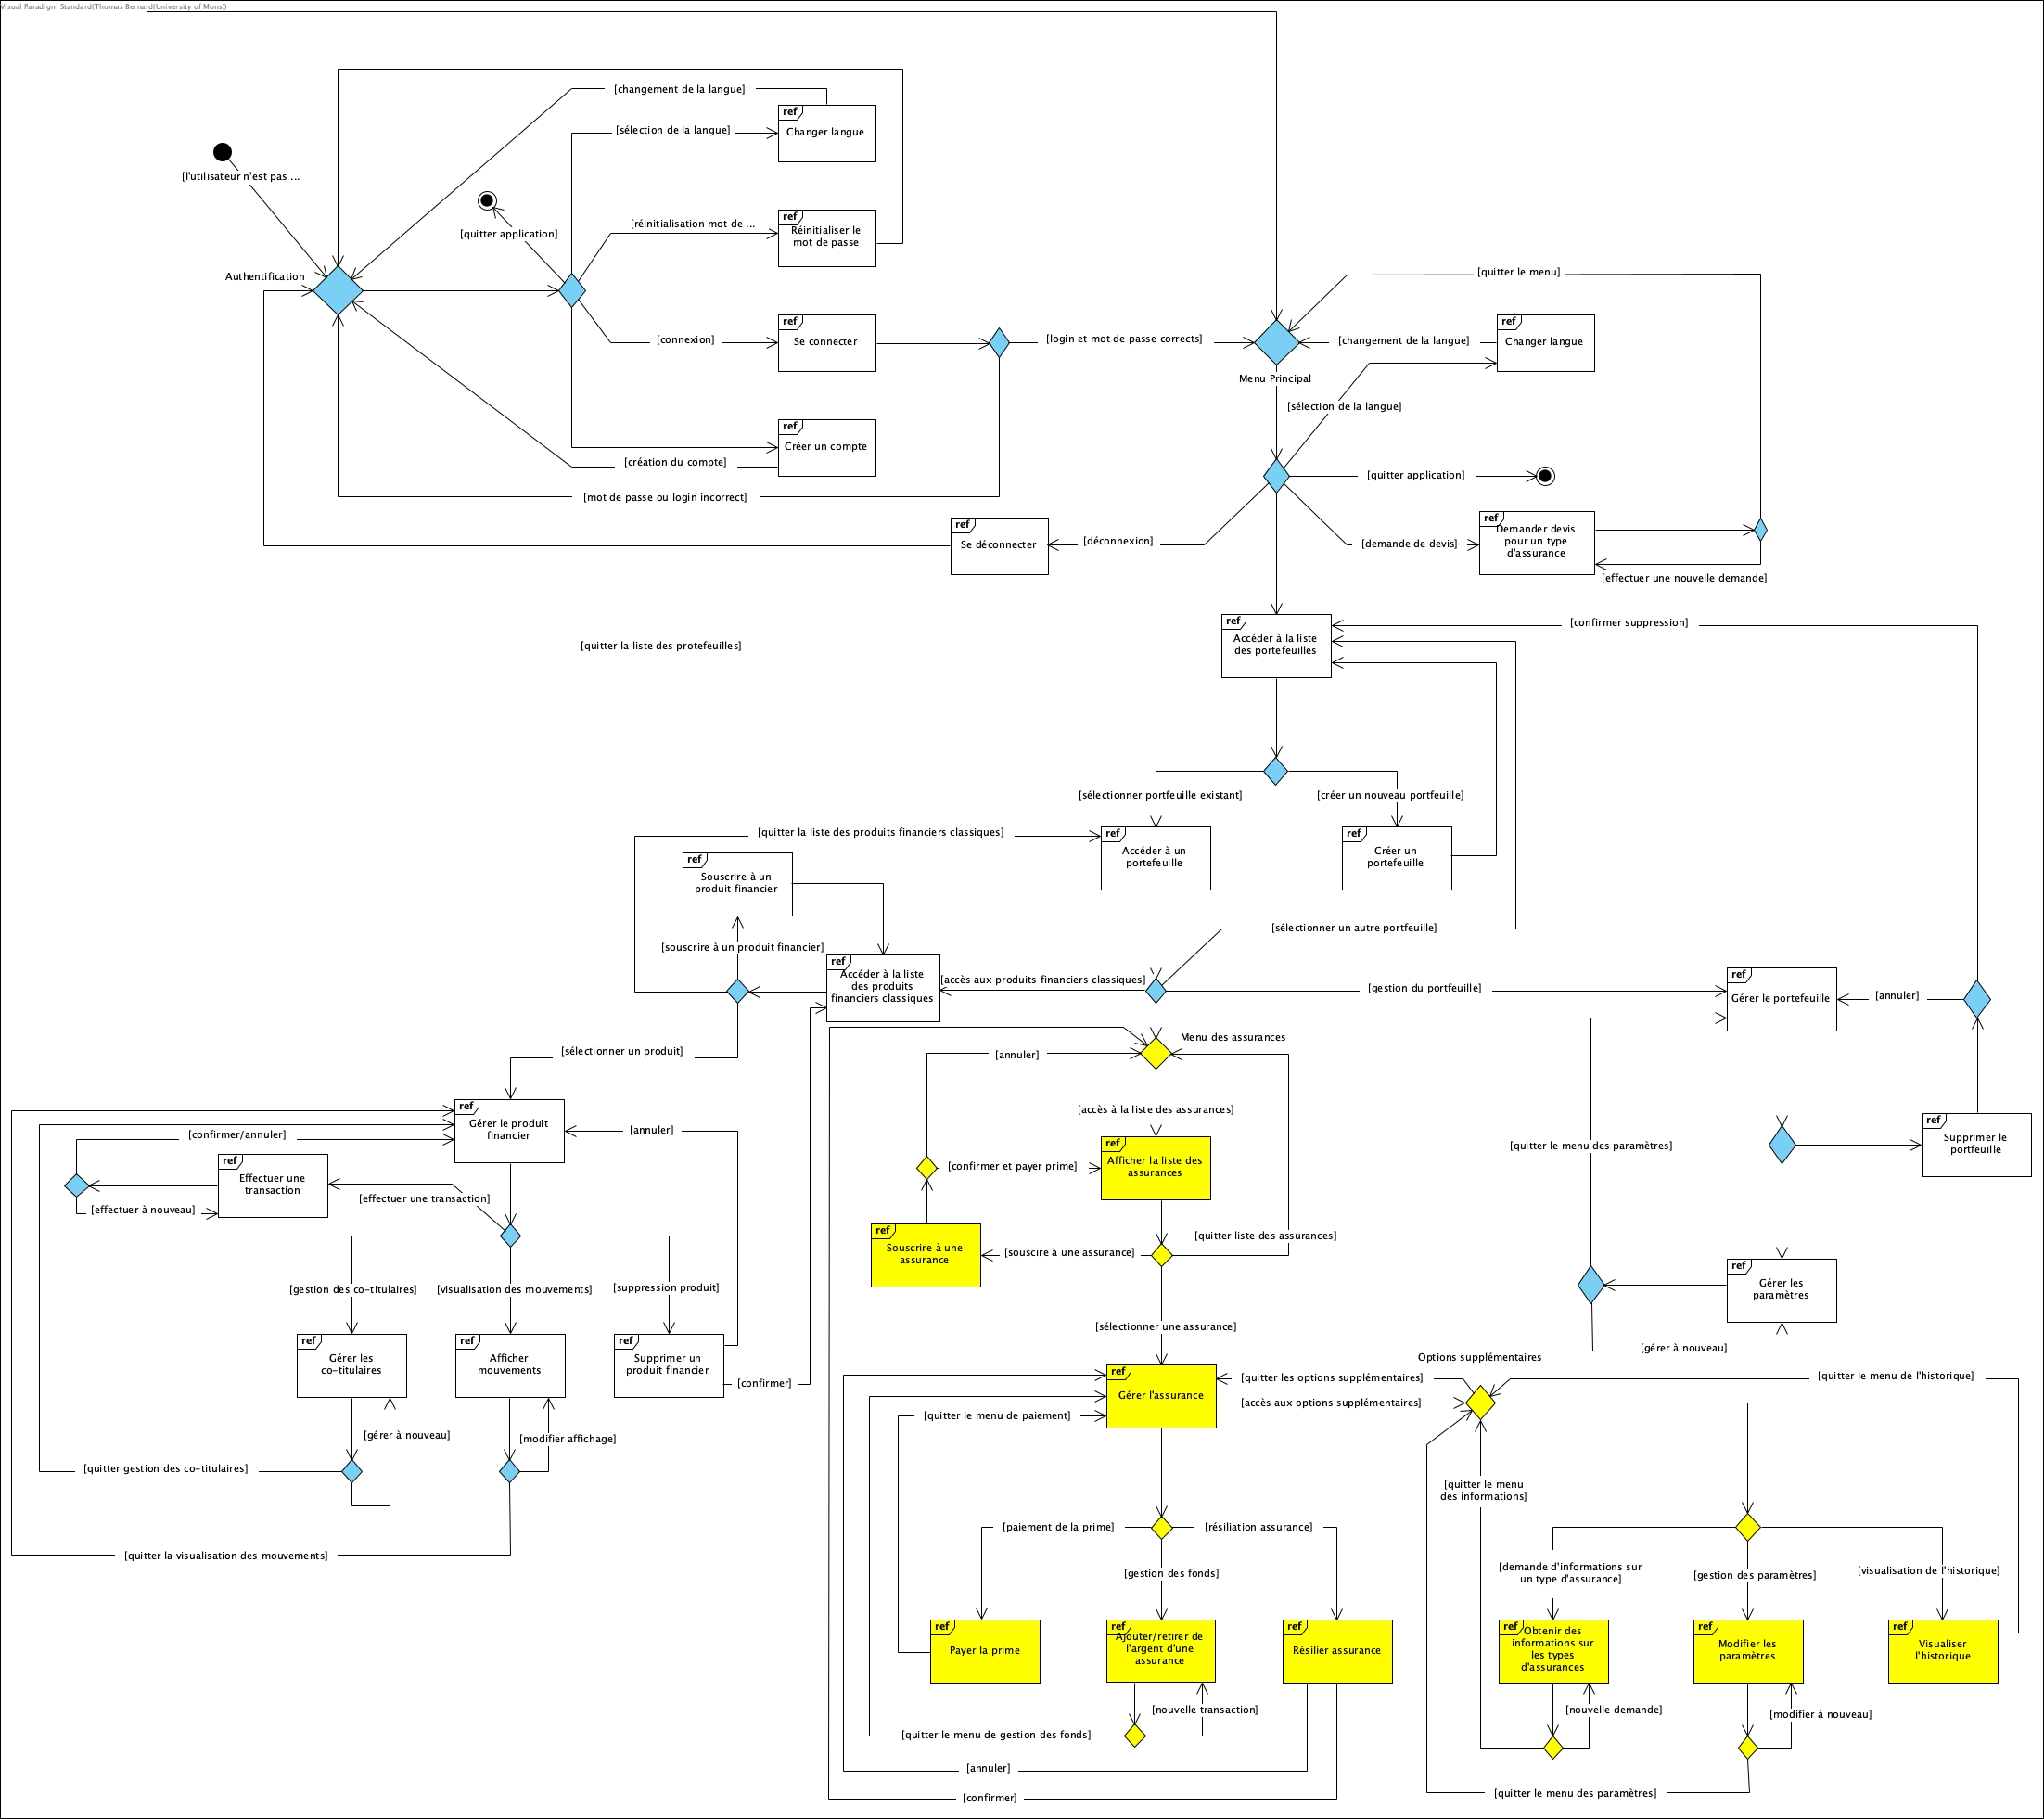
\includegraphics[scale=0.15]{ressources/photos_diagrammes/extensionThomas/intOver1Thomas.jpg}
						\caption{Interaction Overview Diagram de l'app 1 avec extension}
				\end{figure}
		Encore une fois ce diagramme se base sur celui de l'application 1. Notons qu'il est
		maintenant possible de demander un devis depuis le menu principal. Il y a également une 
		différenciation entre les produits financiers classiques et les assurances afin de les 
		séparer en deux scènes différentes plus tard dans la GUI.

\newpage
		\subsubsection{Diagrammes de classe}
				\begin{figure}[h]
						\centering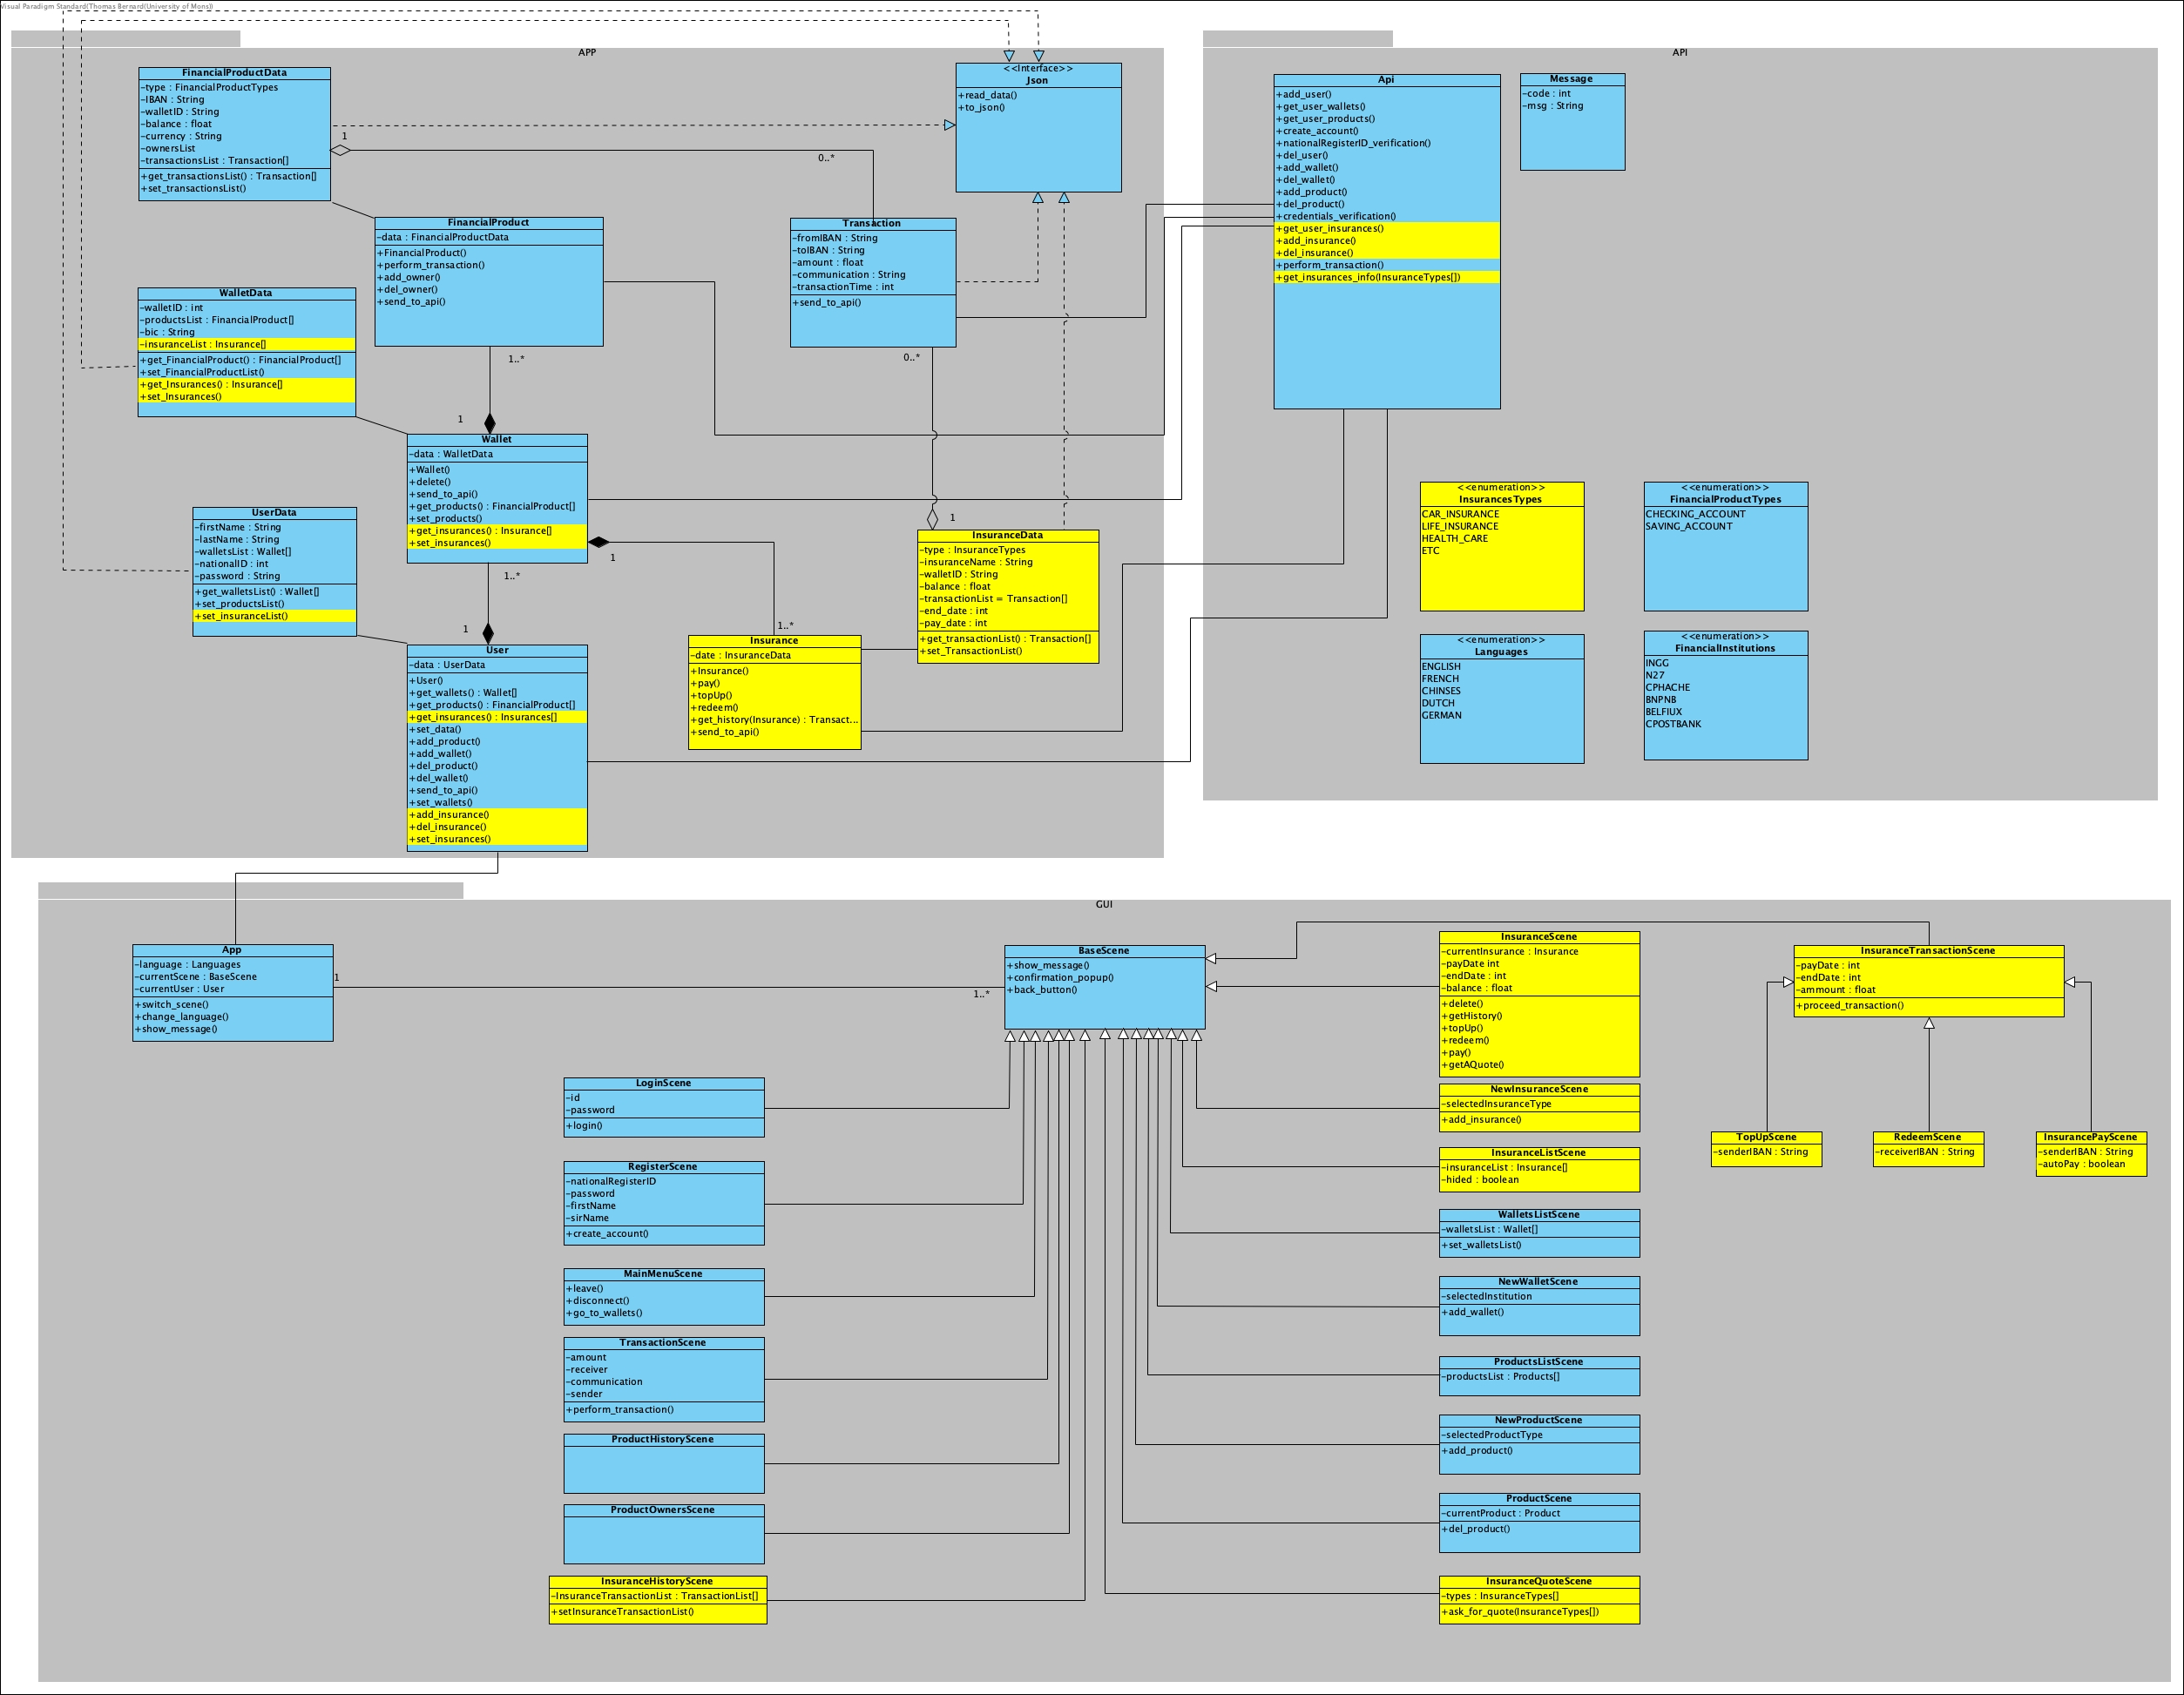
\includegraphics[scale=0.15]{ressources/photos_diagrammes/extensionThomas/class1ExtensionThomas.jpg}
						\caption{Diagramme de classes de l'app 1 avec extension}
				\end{figure}
		Dans la partie logique de l'application (package APP) deux classes ont été rajoutées :
		\textbf{Insurance} et \textbf{InsuranceData}. La première contioent le constructeur et 
		un attribut \textit{data} qui est une objet de type \textit{InsuranceData}. La classe 
		contient également les méthodes liées aux assurances. La classe \textbf{Insurance} est
		liée à la classe wallet de même manière que la classe \textbf{FinancialProduct}. 
		La classe \textbf{Insurance} possède une méthode \textit{send\_to\_api()} et est connectée 
		au package API. La classe \textbf{InsuranceData} implémente l'interface \textbf{Json} qui
		permet d'écrire et le dire des fichiers :json de données et d'ainsir mettre ses données à
		jour.

		\medskip

		Les classes de bases dans lesquelles se trouvaient des listes de produits, des setter et 
		des getter se sont vues ajouter des setter, des getter et des listes mais cette fois-ci
		pour les assurances. 

		\bigskip

		Dans la partie serveur du diagramme de classe (package API) j'ai rajouté une enumération
		\textbf{InsurancesTypes} qui contient les différents types d'assurances afin de pouvoir
		interpréter correctment les données envoyées à la classe \textbf{Api}. Dans la classe
		\textbf{Api} des méthodes ont été rajoutées afin de pouvoir ajouter, supprimer et obtenir
		les assurances d'un client. Il y a également une méthode permettant d'obtenir des 
		informations sur un ou plusieurs types d'assurances dans le cadre de devis.

		\bigskip

		Dans la partie interface graphique (package GUI) il s'agit principalement de nouvelles 
		scènes rajoutées à la manière des scènes de l'application de base. Il n'y a pas de 
		point particulier à expliquer ici.

		\subsubsection{Application 2}

		\subsubsection{Diagramme des cas d'utilisitation}

				\begin{figure}[h]
						\center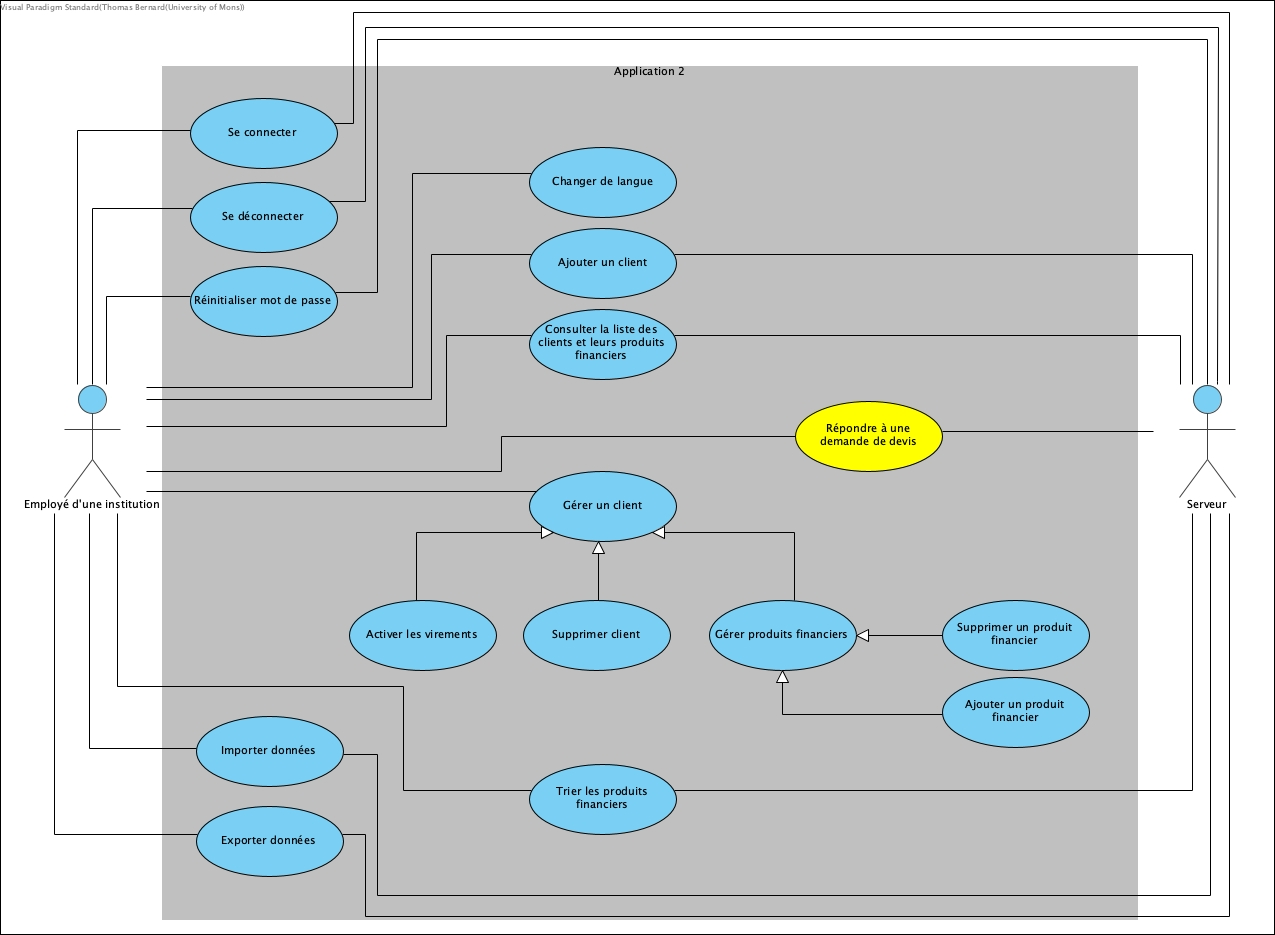
\includegraphics[scale = 0.27]{ressources/photos_diagrammes/extensionThomas/useCase2Thomas.jpg}
						\caption{Diagramme des cas d'utilisation de l'app 2 avec extension}
				\end{figure}

				Le diagramme de cas d'utilisation de l'app 2 ne contient qu'une seule modification.
				Il s'agit du use case permettant de répondre à un devis. En effet lorsqu'une
				institution liste les produits d'un client elle liste également ses assurances.
				Il n'est donc pas nécessaire d'ne rajouter plus.

		\subsubsection{Interaction Overview Diagram}

		Il n'y a également qu'un seul cas d'utilisation rajouté qui est celui de réponse à un
		devis. Par souci de taille du diagramme il n'a pas été ajouté au rapport. L'interaction
		a été rajoutée au niveau du menu de gestion des clients. Une fois l'utilisation terminée,
		le user de l'institution est ramené vers le menu des produits.

		\subsubsection{Diagramme de classes}

				\begin{figure}[h]
						\centering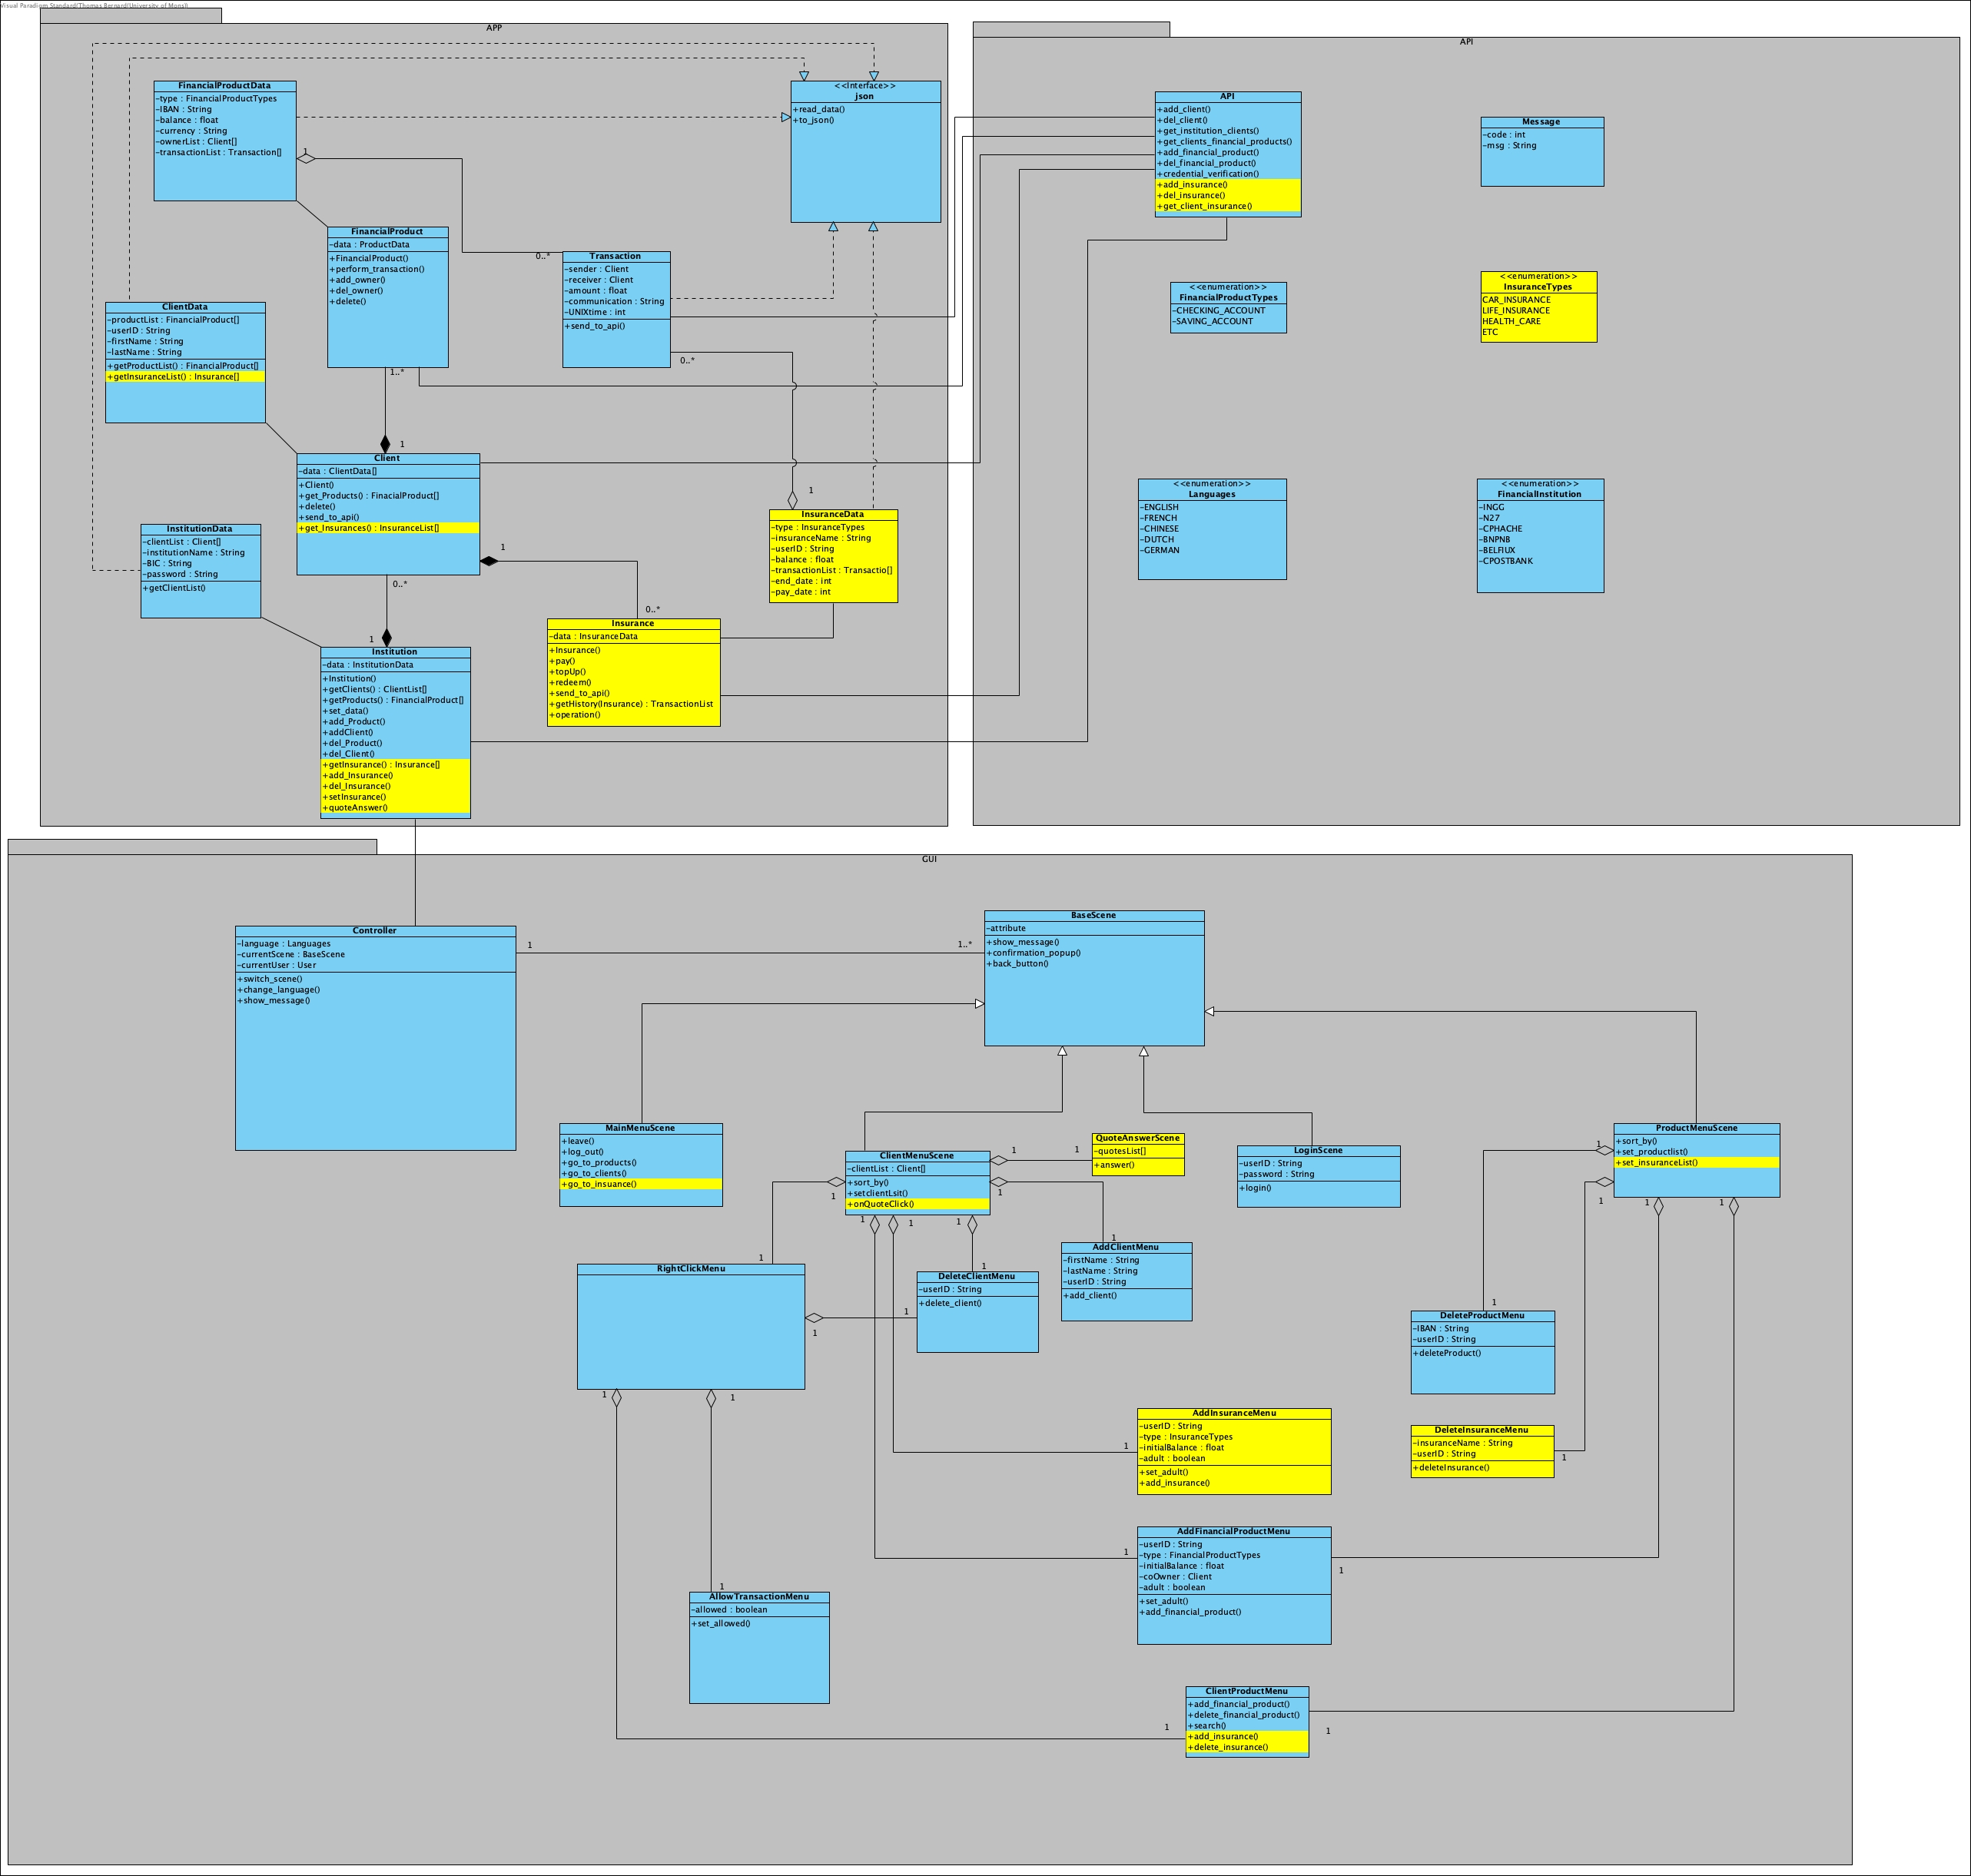
\includegraphics[scale=0.15]{ressources/photos_diagrammes/extensionThomas/class2ExtensionThomas.jpg}
				\end{figure}
		Au niveau de la logique de l'application (package APP) mise à part le fait que la classe 
		\textbf{Insurance} est maintenant reliée à la classe \textbf{Client} du fait que les 
		instituions n'aient pas la notion de portfeuilles et qu'une méthode \textit{quoteAnswer()}
		ait été rajoutée à la classe \textbf{Institution} permettant d'envoyer le devis au client,
		il n'y a pas de changements importants par rapport à celui de l'application 1. 

		\bigskip

		Au niveau de la partie serveur de l'application (package API) le seul cahnegement à noter
		est l'ajout d'une méthode \textit{answerQuote()} dans la classe \textbf{Api} qui permet
		à l'API de générer des réponses à une demande de devis.

		\bigskip

		Au niveau de la partie interface graphique de l'application (package GUI). Une méthode 
		permettant d'accéder à la scène liée aux assurances a été ajoutée à la classe 
		\textbf{MainMenuScene} et une méthode permettant d'accéder à la scène de demande des devis
		a été ajoutée dans la classe \textbf{ClientMenuScene}. Enfin une méthode permettant 
		d'afficher les assurances des clients a été ajoutée à la classe \textbf{ProductMenuScene}.

		\medskip

		Pour ce qui est des classes ajoutées, elles sont au nombre de 3.\\
		Il s'agit des classes suivantes :
		\begin{enumerate}
				\item \textbf{QuoteAnswerScene:} qui est la scène où toutes les demandes de devis
						sont listées et qui contient un bouton permettant d'y répondre.
				\item \textbf{AddInsuranceMenu} cette scène permet d'ajouter une assurance pour
						un client en particulier
		\end{enumerate} 
\newpage

		\subsubsection{Serveur}
		\subsubsection{Diagramme d'entité relation}

				\begin{figure}[h]
						\centering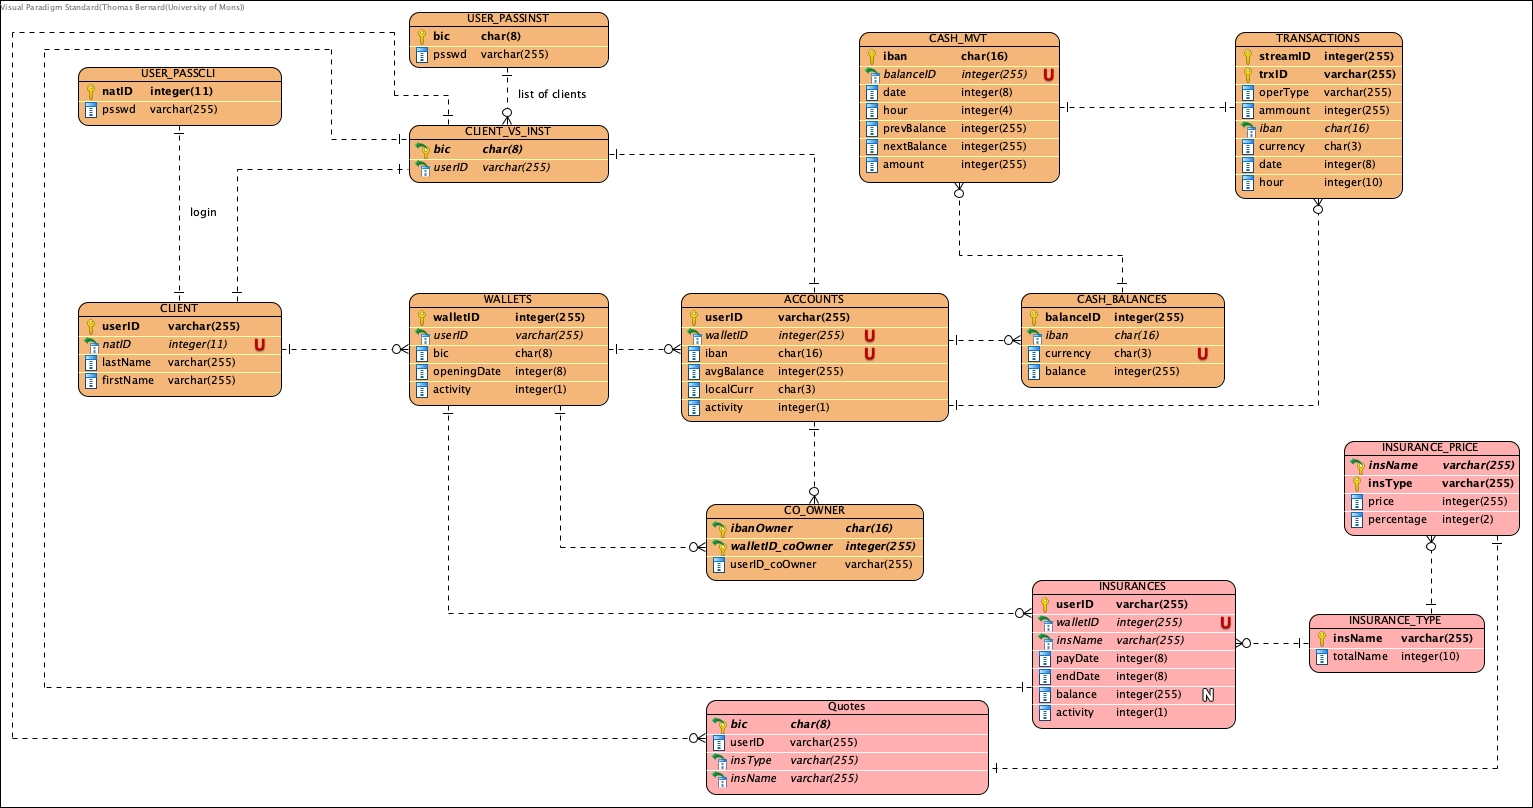
\includegraphics[scale=0.25]{ressources/photos_diagrammes/extensionThomas/erdThomas.jpg}
						\caption{Diagramme d'entité relation avec extension}
				\end{figure}
		Le diagramme d'entité relation a été étendu à l'aide de 3 tables : \textit{INSURANCES, ISNURANCE\_TYPE et INSURANCE\_PRICE}.
				
		\medskip

		La table \textit{INSURANCES} contient toutes les assurances des clients. Elle peut être accédée par 2 tables : par la table \textit{WALLETS} grâce au walletID qui lui est lié dans le cadre de l'application client et par la table \textit{CLIENT\_VS\_INST} grâce au userID qui est lié à chaque assurances dans le cadre de l'application insitution.

		\medskip

		La table \textit{INSURANCE\_TYPE} est une table intermédiaire contenant toutes les assurances proposées dans l'application. On peut obtenir le type d'une assurance depuis la table \textit{INSURANCES} grâce au insuranceName.

		\medskip

		La table \textit{INSURANCE\_PRICE} contient les informations pratiques liées à chaque type d'assurance. Car un type d'assurance peut avoir plusieurs nom (insName) notamment les assurances vies. Cette table est accessible depuis la table \textit{INSURANCE\_TYPE} grâce au insName.

		\subsubsection{Interface graphique de l'extension}

		Plusieurs scène ont été rajoutées contenant les fonctionnalités de l'extension et des scènes de l'application de base ont été modifiées afin de donner accès à ces nouvelles scènes. 
\end{document}
